%ustawienia
\documentclass[12pt,a4paper]{article}
\usepackage[T1]{fontenc}
\usepackage{mathptmx}
\usepackage[utf8]{inputenc}
\usepackage{amssymb}
\usepackage[polish]{babel}
\usepackage{polski}
\usepackage{amsmath}
\usepackage{amsfonts}
\usepackage[left=3.5cm,right=2cm,top=2.5cm,bottom=2.5cm]{geometry}
\usepackage{graphicx}
\usepackage{indentfirst} 
\usepackage{float}
\usepackage{hyperref}
\usepackage[most]{tcolorbox}
\usepackage{fancyhdr}
\setlength{\parindent}{0.7cm}
\hypersetup{
	colorlinks = true,
	linkcolor = black,
	filecolor = magenta,
	urlcolor = blue,
	}
\urlstyle{same}	
	
\author{
	\\\includegraphics[width=0.7\linewidth]{img/logoPWSZ.eps} \\\\\\\\
	\hfill Karpiński Maciej\\
	\hfill Krysa Marcin\\
	\hfill Kuczma Łukasz\\
	\hfill Mertuszka Adam\\\\
	\hfill Prowadzący mgr inż. Marcin Tracz
	}
\title{\textbf{Wprowadzenie do zarządzania projektami deweloperskimi}\\\line(1,0){400}\\\textbf{laboratorium}}
\date{}

\begin{document}

	%Stron tytułowa
	\maketitle
	\thispagestyle{fancy}
	\fancyhf{}
	\rhead{\textcolor{gray}{\footnotesize Państwowa Wyższa Szkoła Zawodowa im. Witelona w Legnicy\\Informatyka, rok III\\Semestr zimowy 2020/2021}}	
	\renewcommand{\headrulewidth}{0pt}
	\clearpage

	%Spis treści
	\pagestyle{fancy}
	\rfoot{\thepage}	
	\tableofcontents
	\newpage

	%opis projektu
	\section{Opis projektu}
		\indent Projekt ,,Magazynek piwosza'' jest aplikacją internetową przeznaczoną dla pasjonatów warzących piwo w domu, którzy chcieliby posiadać listę posiadanych składników.
		,,Magazynek piwosza'' pozwala zarejestrowanemu i zalogowanemu użytkownikowi na tworzenie swoich wirtualnych ,,schowków'' i przypisywania do nich
		składników wraz z ich datami ważności. Funkcjonalność aplikacji obejmuje:
		\begin{itemize}
			\item Dostęp do aplikacji poprzez przeglądarkę www (PC, smartphone)
			\item rejestrację i logowanie użytkowników,
			\item dodawanie, modyfikowanie i usuwanie kategorii przedmiotów,
			\item dodawanie, modyfikowanie i usuwanie przedmiotów,
			\item dodawanie, modyfikowanie i usuwanie magazynów,
			\item wysyłanie powiadomień o zbliżającym się terminie ważności,
		\end{itemize}		
	\newpage
	
	%Opis poszczególnych ról w grupie, kto za co był odpowiedzialny
	\section{Role w grupie}
	\indent Każdy z członków zespołu posiada następujące role:
	\begin{itemize}
		\item Karpiński Maciej:
			\begin{itemize}
				\item Backend
				\item Baza danych
				\item DevOps
				\item Dokumentacja
				\item Testy integracyjne
			\end{itemize}
		\item Krysa Marcin
			\begin{itemize}
				\item Frontend
			\end{itemize}
		\item Kuczma Łukasz
			\begin{itemize}
				\item Backend
			\end{itemize}
		\item Mertuszka Adam
			\begin{itemize}
				\item Frontend
				\item Lider
				\item Project Manager
			\end{itemize}
	\end{itemize}		
	\newpage
	
	%Opis wymagań i założeń projektowych
	\section{Wymagania i założenia projektowe}
		Wymagania projektowe:
		\begin{itemize}
			\item Uwierzytelnianie (w tym poprzez social media);
			\item Przechowywanie różnych typów produktów;
			\item Powiadomienia;
			\item Poręczny interfejs;
			\item Separacja backendu i frontendu;
			\item Logi.
		\end{itemize}
		Założenia:
		\begin{itemize}
			\item Użytkownik może tworzyć swoje własne schowki;
			\item Użytkownik wybiera składnik z listy składników i dodaje go do swojego schowka;
			\item Użytkownik wprowadza termin ważności składnika;
			\item Użytkownik dostaje powiadomienie o zbliżającym się terminie ważności;
			\item Przyjazny interfejs użytkownika;
		\end{itemize}				 
	\newpage
	
	%Opis działania aplikacji / systemu
	\section{Opis działania}

	\indent Aplikacja pierwotnie stworzona dla miłośników piwowarstwa, ma za zadanie pomóc w zarządzaniu składnikami w swoich magazynkach, które niezbędne są do warzenia piwa. 
Wszystkie dodane magazyny są indywidualne i spersonalizowane, stąd też program wymaga od użytkownika zalogowania się albo poprzez rejestrację na stronie, albo używając mediów społecznościowych (gmail, facebook).
Aby użytkownik dodał swoje produkty, musi na samym początku dodać swój pierwszy magazyn. Składów może być wiele - użytkownik może je podzielić wedle uznania kategoriami lub użyć jednego magazynu, aby trzymać w nim wszystkie składniki.
\newline \indent Każdy produkt posiada swoją indywidualną datę przydatności do spożycia, dlatego też przy dodawaniu przedmiotu do magazynu, niezbędne jest podanie daty przydatności do spożycia. 
\newline \newline \indent Aplikacja raz dziennie zbiera wszystkie informacje na temat produktów dodanych w magazynach, sprawdza daty przydatności i wysyła spersonalizowane powiadomienia mailowe z informacją, który składnik przeterminuje się lub który już jest przeterminowany. 
\newline \newline \indent Gotowa aplikacja przystosowana będzie typowo pod miłośników piwowarstwa, więc użytkownicy, przy dodawaniu przedmiotów do swoich magazynów, będą mogli wybierać predefiniowane składniki tylko z kategorii ''Piwowarstwa'', jednak aplikacja zostanie stworzona w taki sposób, aby umożliwić przyszłościowo rozbudowanie blibliotek produktowych o np. ''nabiał'', czy ''produkty mięsne''.
	%Opis wykorzystanych technologii, narzędzi i rozwiązań technicznych
	\newpage
	\section{Wykorzystana technologia i narzędzia}
	\indent skopiować finalny
	\newpage

	%Opis event stormingu + zrzuty z modelowania (wyraźne)
	\section{Event storming}
		\indent Event Storming został przeprowadzony na portalu ,,Miro'' \url{https://miro.com/}, w dniu 13.12.2020 było to nowe i ciekawe doświadczenie dla każdego z członków zespołu.
		Projekt w momencie przeprowadzenia event stormingu był już w zaawansowanej formie, wraz z rozpisanymi zadaniami więc wykorzystaliśmy spotkanie
		do stworzenia modelu pracy aplikacji.\\
		\indent Podczas tworzenia wizualizacji okazało się, że rozumienie aspektów działania i reagowania aplikacji na niektóre zdarzenia
		różnią się między poszczególnymi członkami zespołu, ujawnione różnice w wyobrażeniu na temat funkcjonowania poszczególnych komponentów aplikacji spowodowały dyskusje
		nad wyborem najlepszego rozwiązania. Podczas spotkania wyraźnie było widać brak doświadczenia w tego typu zadaniu, na początku często przerywaliśmy sobie wypowiedzi ale dość szybko
		doszliśmy do porozumienia i zapanował porządek. W miarę rozwoju aplikacji do modelu były dodawane kolejne szczegóły. 
		Wynikiem event stormingu jest spójny model działania aplikacji, dzięki czemu każdy członek zespołu może prześledzić przepływ informacji.
		\begin{figure}[H]
			\centering
			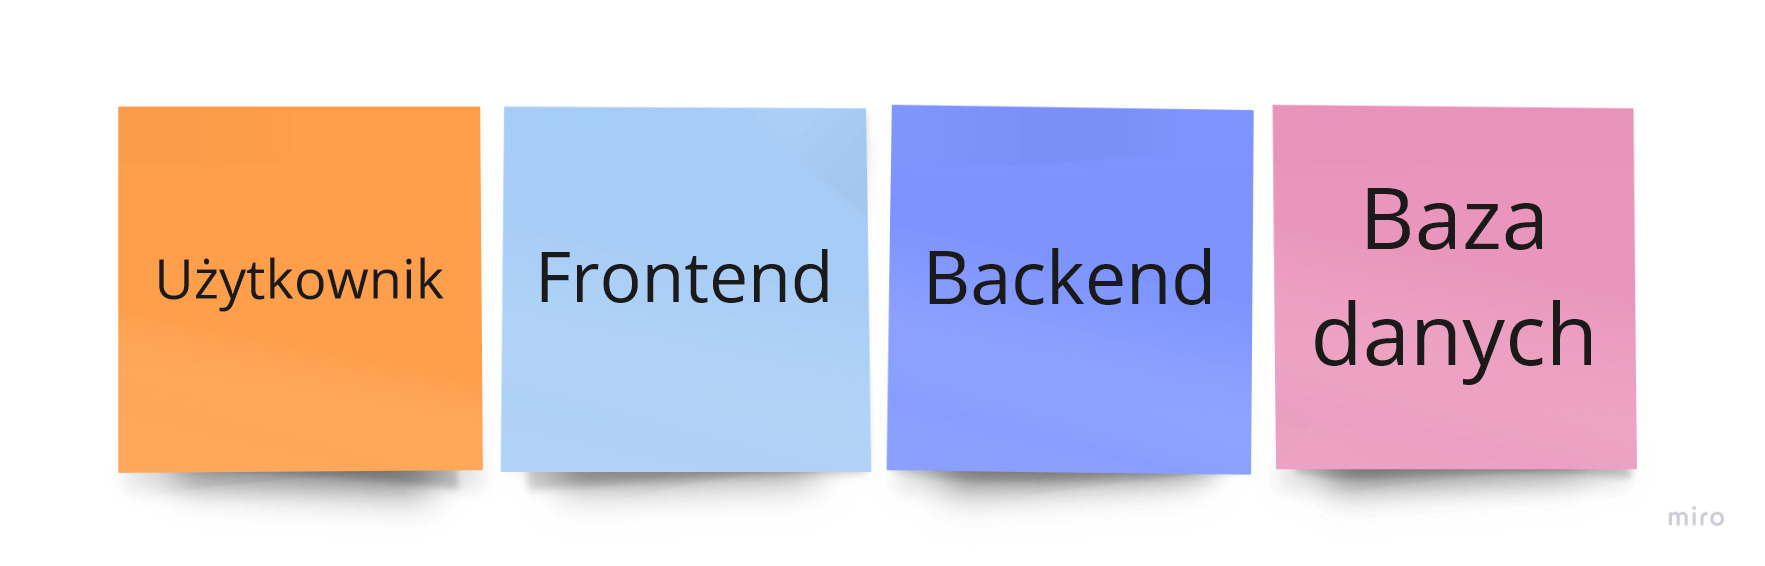
\includegraphics[width=0.6\textwidth]{img/miro_2.jpg}
			\caption{Miro - Legenda}
			\label{fig:miro-legenda}
		\end{figure}				
		\begin{figure}[H]
			\centering
			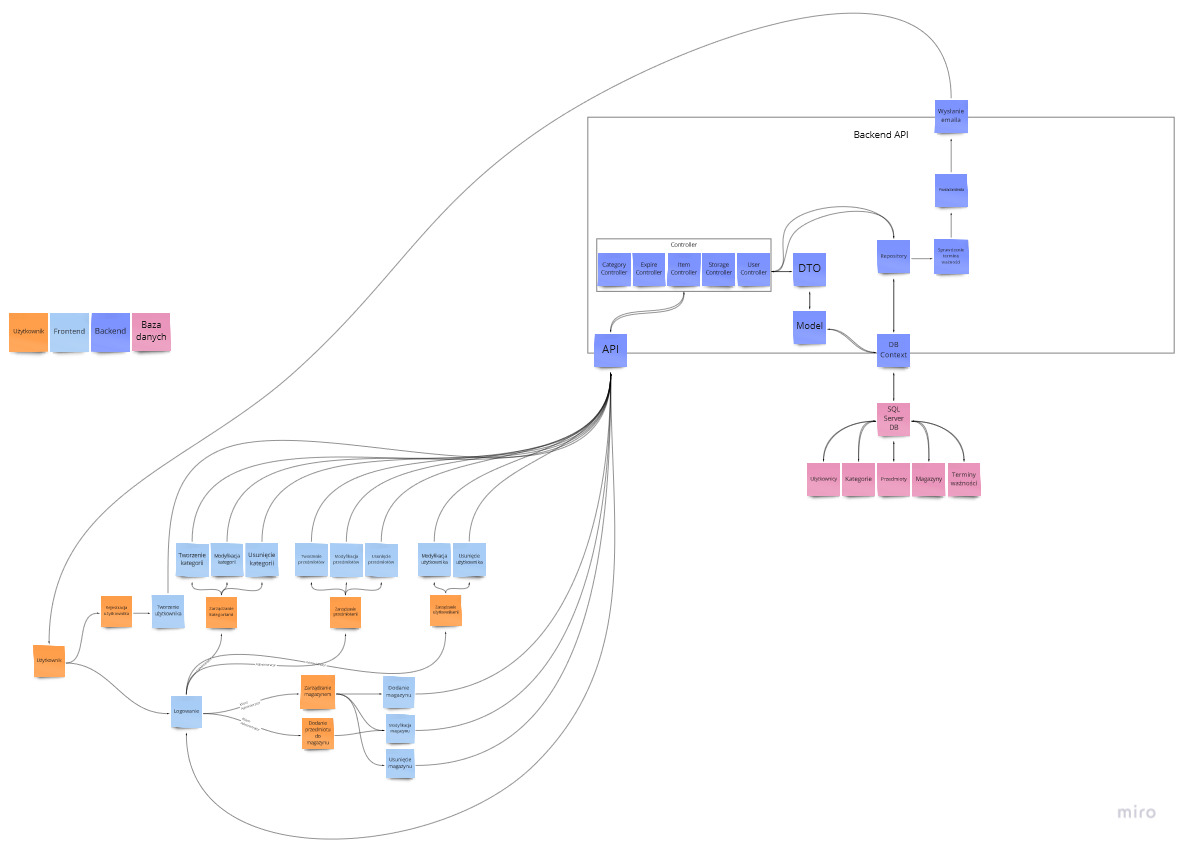
\includegraphics[width=\textwidth]{img/miro_1.jpg}
			\caption{Miro - Schemat działania aplikacji}
			\label{fig:miro-ogolne}
		\end{figure}
		\begin{figure}[H]
			\centering
			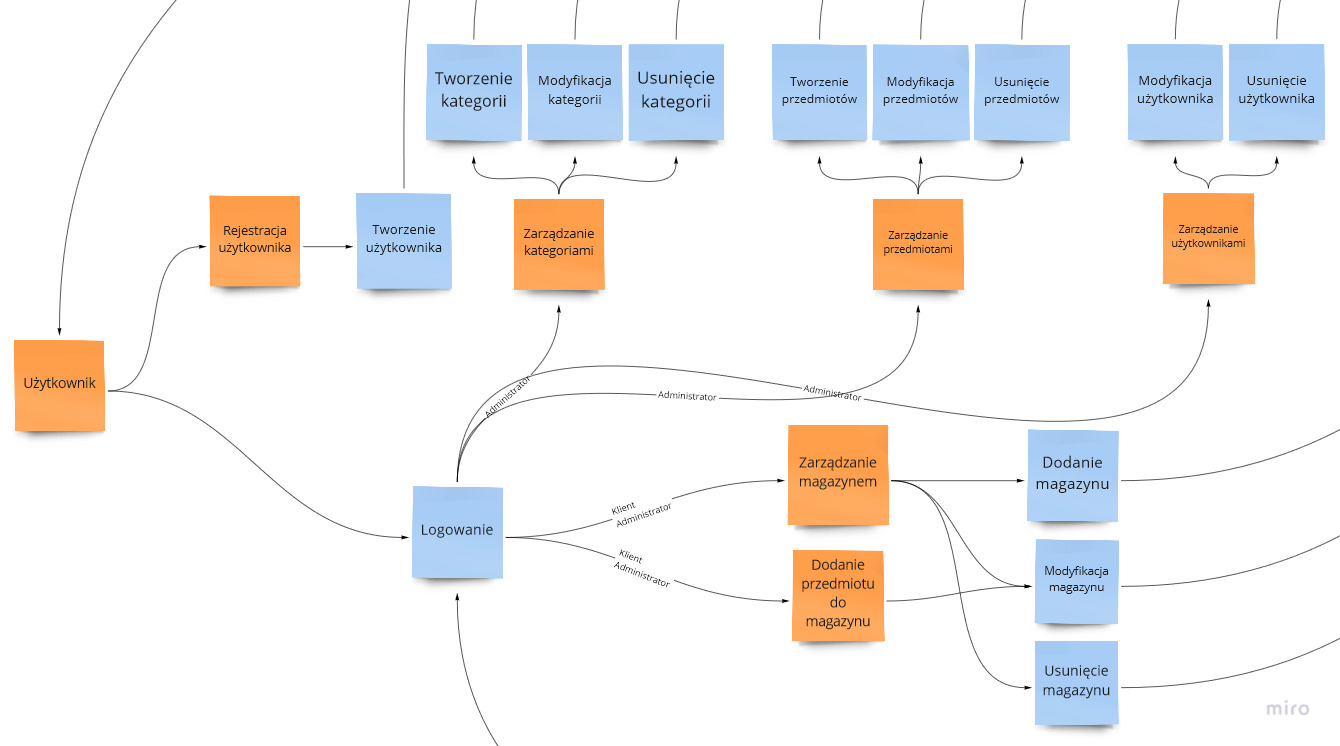
\includegraphics[width=\textwidth]{img/miro_4.jpg}
			\caption{Miro - Frontend aplikacji}
			\label{fig:miro-front}
		\end{figure}
		\begin{figure}[H]
			\centering
			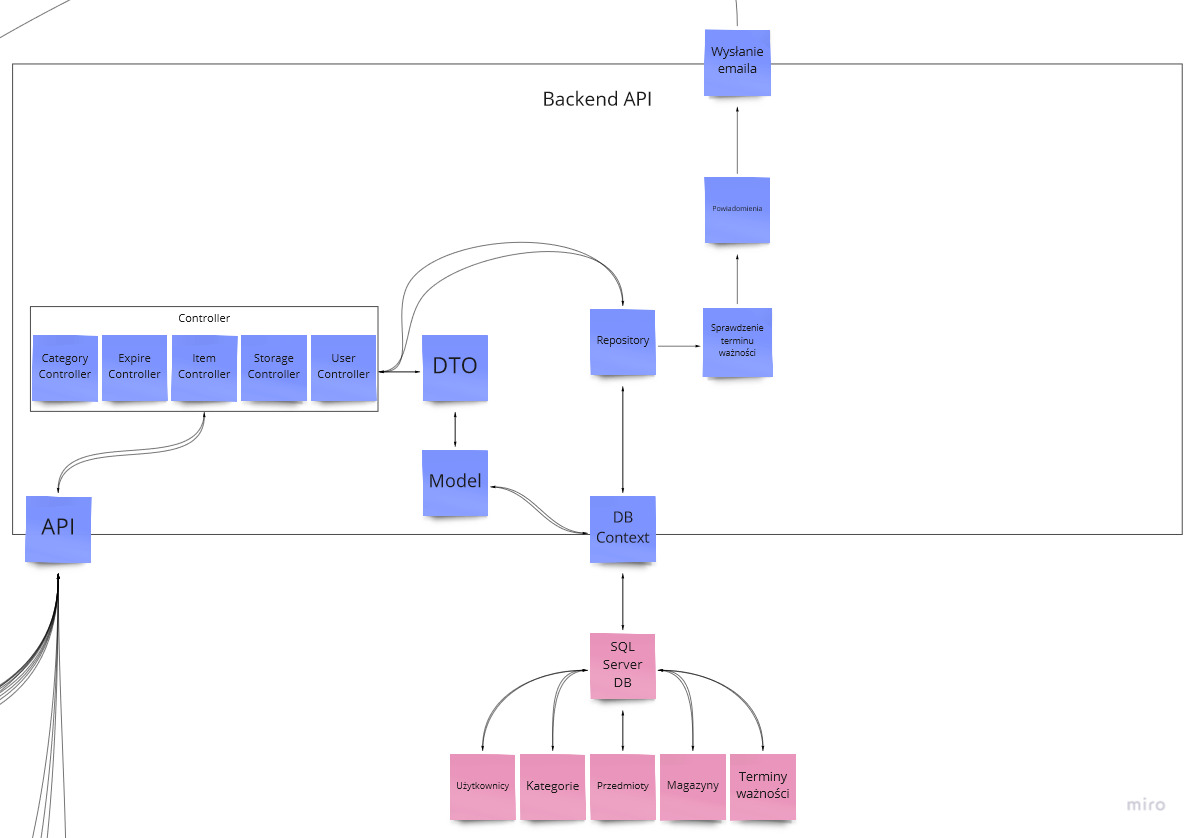
\includegraphics[width=\textwidth]{img/miro_3.jpg}
			\caption{Miro - Backend aplikacji}
			\label{fig:miro-backend}
		\end{figure}
	\newpage
	
	%Backlog
	\section{Backlog}
		\indent Backlog zaplanowanych działań został rozpisany na platformie ,,Trello'', pod adresem: \url{https://trello.com/b/z9uj9uzc}
		\newline
		\begin{figure}[H]
			\centering
			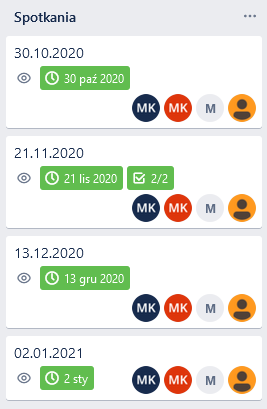
\includegraphics[width=0.3\textwidth]{img/spotkania.png}
			\caption{Terminy spotkań}
			\label{fig:trello-spotkania}
		\end{figure}
		
	\newpage
	
	%Estymata
	\section{Estymata}
		\indent Szacowana estymacja poszczególnych części realizacji projektu:
		\begin{itemize}
			\item Backend:
				\begin{itemize}
					\item Autoryzacja: 10 godzin,
					\item Data Transfer Object (DTO): 2 godziny,
					\item DevOps: 5 godzin,
					\item End Point: 15 godzin,
					\item Harmonogram: 3 godziny,
					\item Logi: 10 godzin,
					\item Programowanie logiki aplikacji: 50 godzin,
					\item SQL Repozytorium: 3 godziny,
					\item Testy integracyjne: 10 godzin,
					\item Uwierzytelnianie: 10 godzin, 
					\item Wysyłanie e-maili: 30 minut,
				\end{itemize}
			\item Baza danych:
				\begin{itemize}
					\item Konfiguracja: 30 minut,
					\item Projekt tabel: 2 godziny,
				\end{itemize}
			\item Dokumentacja projektu: 5 godzin,
			\item Frontend: 
				\begin{itemize}
					\item DevOps: 3 godzinny,
				\end{itemize}
			\item Zarządzanie projektem:
				\begin{itemize}
					\item Rozpisanie backlogu: 2 godziny,
					\item Rozpisanie sprintów: 2 godziny,
				\end{itemize}
		\end{itemize}				

	\newpage

	%Opis sprintów + zrzuty
	\section{Sprinty}
		\indent Ze względu na różne harmonogramy pracy zawodowej poszczególnych członków zespołu, trudno było wyznaczyć szczegółowy termin realizacji pojedynczych komponentów aplikacji,
		więc zostały wyznaczone jedynie ostateczne terminy elementów, na których bazują inne części aplikacji. Pozostałe elementy były realizowane w drugiej kolejności.\\
		\indent Backend:
		\begin{figure}[H]
			\centering
			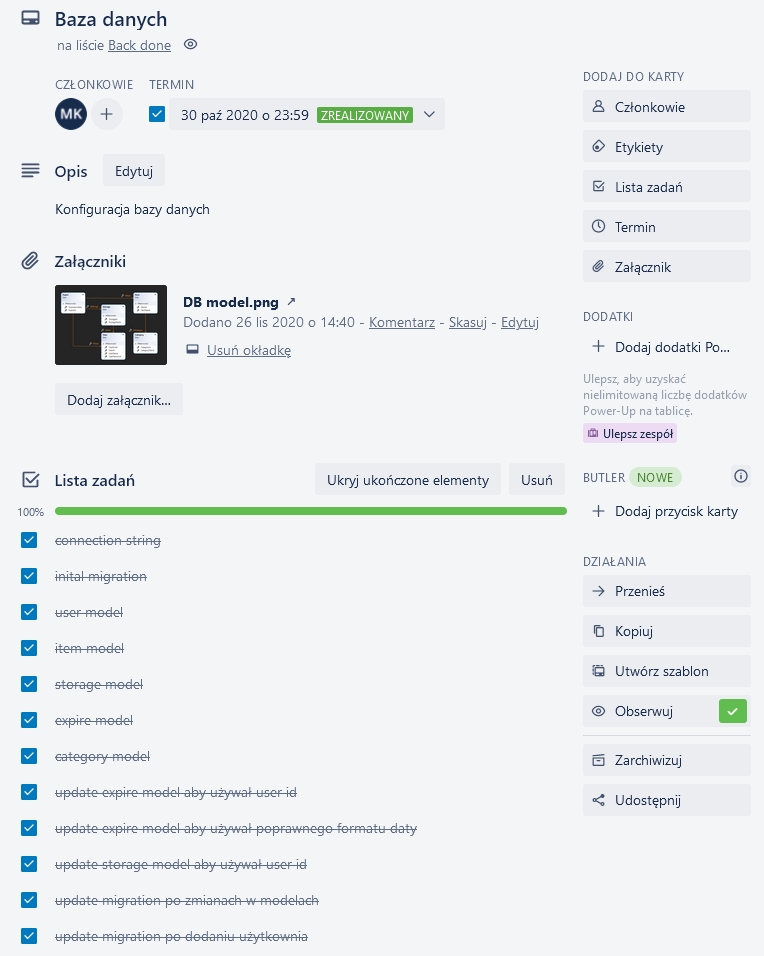
\includegraphics[width=\textwidth]{img/DBSprint.png}
			\caption{Sprinty - Baza danych}
			\label{fig:sprint-db}
		\end{figure}
				\begin{figure}[H]
			\centering
			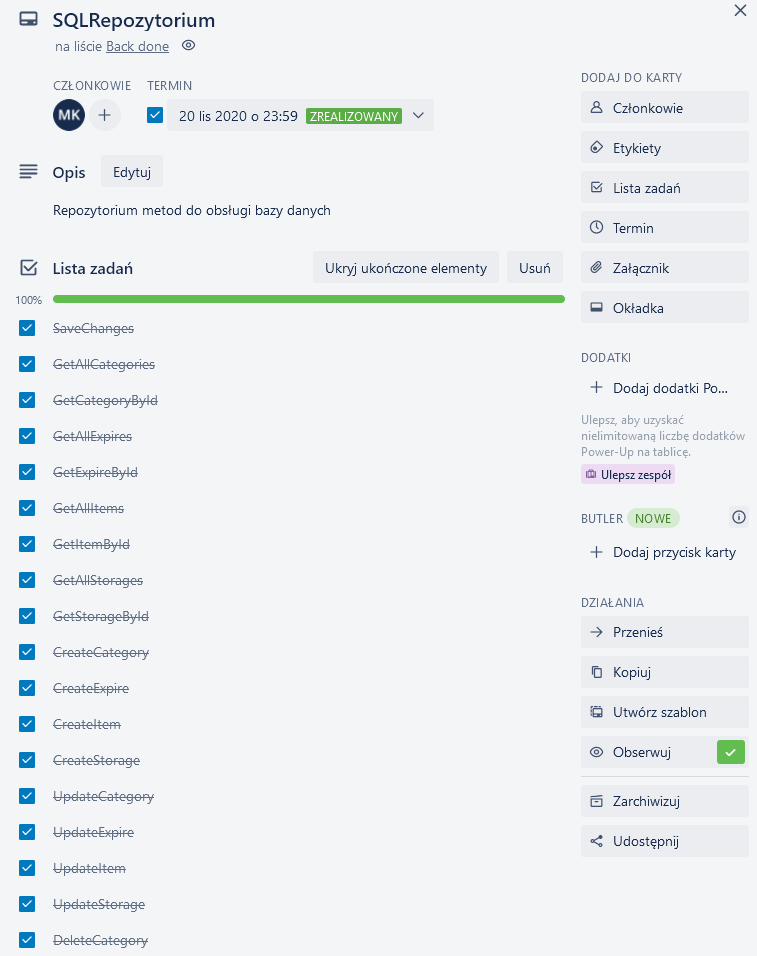
\includegraphics[width=\textwidth]{img/SQLRepo_Sprint.png}
			\caption{Sprinty - Repozytorium SQL}
			\label{fig:sprint-SQLRepo}
		\end{figure}
				\begin{figure}[H]
			\centering
			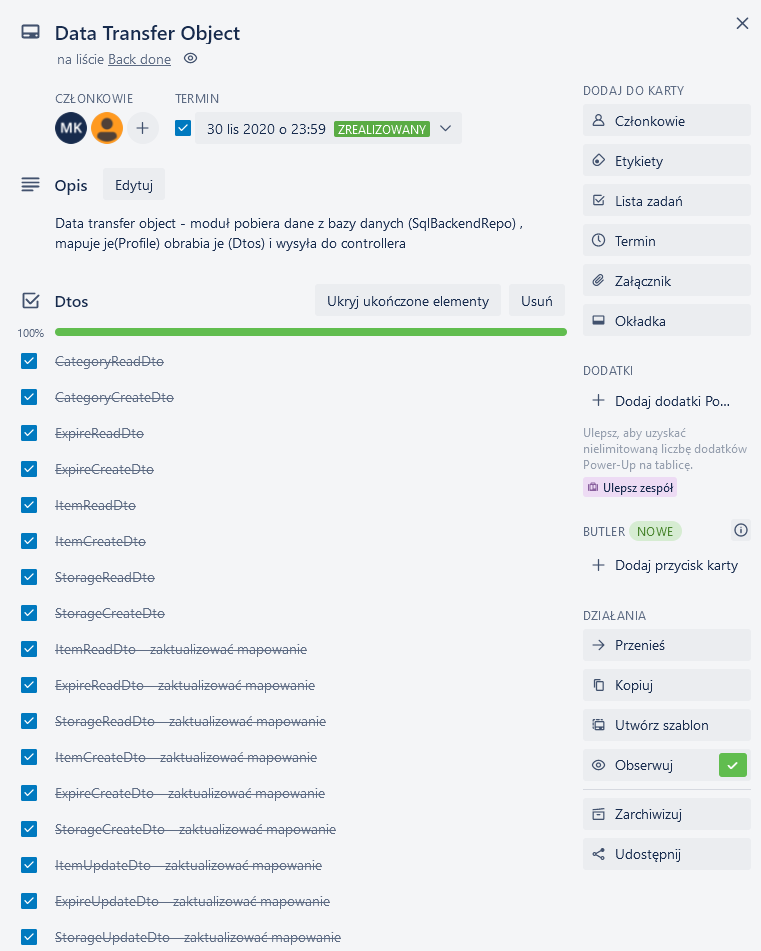
\includegraphics[width=\textwidth]{img/DTO_Sprint.png}
			\caption{Sprinty - Data Transfer Object}
			\label{fig:sprint-dto}
		\end{figure}
				\begin{figure}[H]
			\centering
			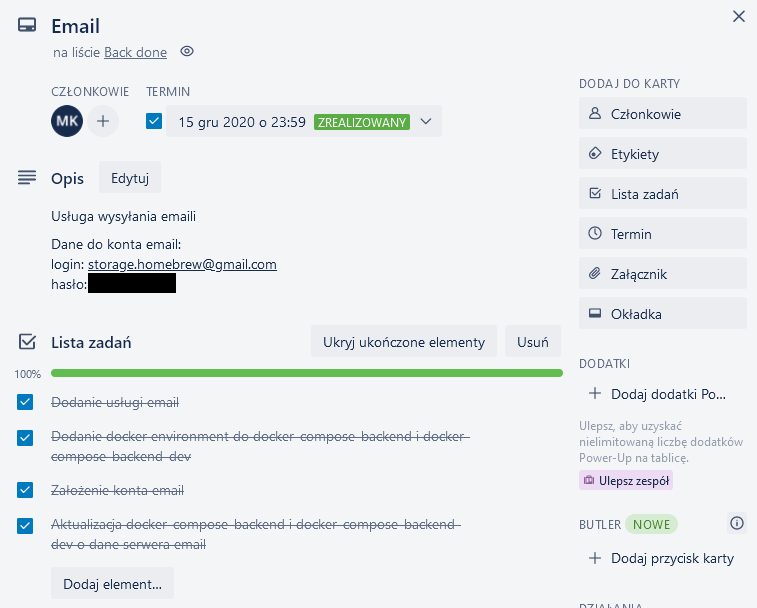
\includegraphics[width=\textwidth]{img/Email_sprint.png}
			\caption{Sprinty - usługa wysyłania e-maili}
			\label{fig:sprint-email}
		\end{figure}
	\newpage
	
	%Interfejs aplikacji (zrzuty) + krótki opis
	\section{Interfejs aplikacji}
	\newpage
	
	%Informacje uruchomieniowe w środowisku developerskim (instrukcja, co zrobić aby po ściągnięciu projektu z repozytorium GIT, móc uruchomić go na lokalnej maszynie)
	\section{Uruchomienie w środowisku developerskim}
		\indent Repozytorium kodu projektu i jego dokumentacja znajdują się w serwisie ,,GitHub'' pod adresem: 
			\begin{tcolorbox}[minipage,colback=white,arc=0pt,outer arc=0pt, fontupper=\scriptsize]
				\center
				\url{https://github.com/MacKarp/Homebrewing-storage}
			\end{tcolorbox}
		\indent Do uruchomienia systemu wymagana jest działająca platforma konteneryzacji ,,Docker''
			oraz narzędzie ,,Docker Compose'' szczegóły instalacji i konfiguracji wymaganych
			komponentów, można sprawdzić na stronie internetowej: \url{https://docs.docker.com/}.\\
		\indent Po ściągnięciu repozytorium w katalogu głównym projektu znajdują się pliki wsadowe, umożliwiające kompilację i uruchomienie ,,frontendu'' i ,,backendu''
		wraz z bazą danych.
		Pliki wsadowe dla systemu Windows:
		\begin{itemize}
			\item Backend-Start.bat
			\item Backend-Start-DEV.bat
			\item Backend-Stop.bat
			\item Backend-Stop-DEV.bat
		\end{itemize}
		Pliki dla systemu Linux:
		\begin{itemize}
			\item Backend-Start.sh
			\item Backend-Start-DEV.sh
			\item Backend-Stop.sh
			\item Backend-Stop-DEV.sh
		\end{itemize}
		Pliki ,,Backend-Start.bat'', ,,Backend-Stop.bat'' oraz ,,Backend-Start.sh'' i ,,Backend-Stop.sh'' służą do uruchomiania i zatrzymywania ,,backendu'' w wersji produkcyjnej,
		która pobierze i~uruchomi najnowszą stabilną wersję ,,backendu'' aplikacji i bazę danych z serwisu ,,Docker Hub'', w przypadku pliku z przyrostkiem ,,DEV''
		zostanie uruchomiona kompilacja wersji deweloperskiej znajdującej się w lokalnym katalogu ,,Backend'' a następnie zostanie utworzony kontener z działającą aplikacją.
		W przypadku chęci zmiany ustawień ,,backendu'' aplikacji lub kontenera należy edytować - zachowując odpowiednie formatowanie plików yaml - plik w wersji produkcyjnej
		lub deweloperskiej:
		\begin{itemize}
			\item docker-compose-backend.yaml
			\item docker-compose-backend-dev.yaml		
		\end{itemize}
	\newpage	
	
	%Podsumowanie, wnioski
	\section{Podsumowanie}
		\indent Sprawne zarządzanie projektem jest trudnym zadaniem i wymaga aby lider projektu był osobą charyzmatyczną.\\
		\indent Zarządzanie zespołem, w którym każdy z członków
		posiada różny harmonogram pracy zawodowej sprawiło wiele problemów organizacyjnych, często każdy z członków zespołu był dostępny w innym terminie,
		przez co ustalenie terminu spotkania online, w którym każdy z członków zespołu byłby dostępny było trudnym zadaniem, z tego powodu w czasie trwania projektu dominowała
		komunikacja pisana. Z tych samych względów rozpisywanie sprintów ograniczyło się jedynie do określenia nieprzekraczalnego terminu ukończenia elementów, od których inne
		komponenty projektowanej aplikacji były uzależnione, pozostałe elementy nie posiadały ściśle określonego terminu i były realizowane w drugiej kolejności.\\
		\indent Każdy z członków zespołu zdobył dużo wiedzy na temat pracy w zorganizowanym zespole, a także poznał narzędzia ułatwiające pracę w takim zespole.\\
		\indent Wspólnie doszliśmy do wniosku że Event Storming był nowym i  ciekawym doświadczeniem, chodź lepszym byłoby spotkanie ,,twarzą w twarz''
		wraz z osobą doświadczoną, która mogłaby poprowadzić takie spotkanie.\\
		\indent Wszyscy członkowie zespołu zgodnie stwierdzili że największym problem podczas pracy był problem z bieżącą komunikacją oraz z początkowym brakiem zrozumienia działania
		tablic na platformie ,,Trello'', raz zdarzyło się nawet	że dwie osoby zrobiły tą samą część aplikacji - na szczęście strata czasu w tym wypadku była mała. 	
\end{document}